
\documentclass[UTF8]{beamer}
\setbeamertemplate{caption}[numbered]
\setbeamertemplate{bibliography item}[text]
%\addtobeamertemplate{note page}{}{\thispdfpagelabel{notes:\insertframenumber}}
\mode<presentation> {
\usetheme{Madrid}
}
\usepackage{graphicx} % Allows including images
\usepackage{booktabs} % Allows the use of \toprule, \midrule and \bottomrule in tables
%\usepackage{ctex}
\usepackage{ragged2e}
\usepackage{multirow}

\justifying\let\raggedright\justifying
                             
%----------------------------------------------------------------------------------------
%	TITLE PAGE
%----------------------------------------------------------------------------------------
\title[Volume: 9 Issue: 14] %optional
{Toward Crowdsourced Transportation \\Mode Identification: A Semisupervised Federated Learning Approach}

%\subtitle{A short story}

\author[IEEE Internet of Things Journal] % (optional, for multiple authors)
{Reporter: Qihan Huang\\  Supervisor: Jing Zhang
}

\date[10.1109/JIOT.2021.3132056]{November 16, 2022}
\titlegraphic{\includegraphics[width=2cm]{images/logo.png}}


%----------------------------------------------------------------------------------------
%	Highlight the title of the current section
%----------------------------------------------------------------------------------------
\AtBeginSection[]
{
  \begin{frame}
    \frametitle{Outline}
    \tableofcontents[currentsection]
  \end{frame}
}


%----------------------------------------------------------------------------------------
%	All pages in the slides
%----------------------------------------------------------------------------------------
\begin{document}

% insert title page---------------------------
\frame{\titlepage}

%insert contents------------------------------
\begin{frame}
\frametitle{Outline}
\tableofcontents
\end{frame}

%insert introduction--------------------------
\section{Introduction}

\begin{frame}
\frametitle{Background}
\begin{columns}

\column{0.5\textwidth}
Privacy-preserving transportation mode identification (TMI) is among the key challenges toward future intelligent transportation systems. With recent developments in federated learning (FL), crowdsourcing has emerged as a promising costeffective data source for training powerful TMI classifiers without compromising users’ data privacy. 


\column{0.5\textwidth}
\begin{figure}[ht]
\centering
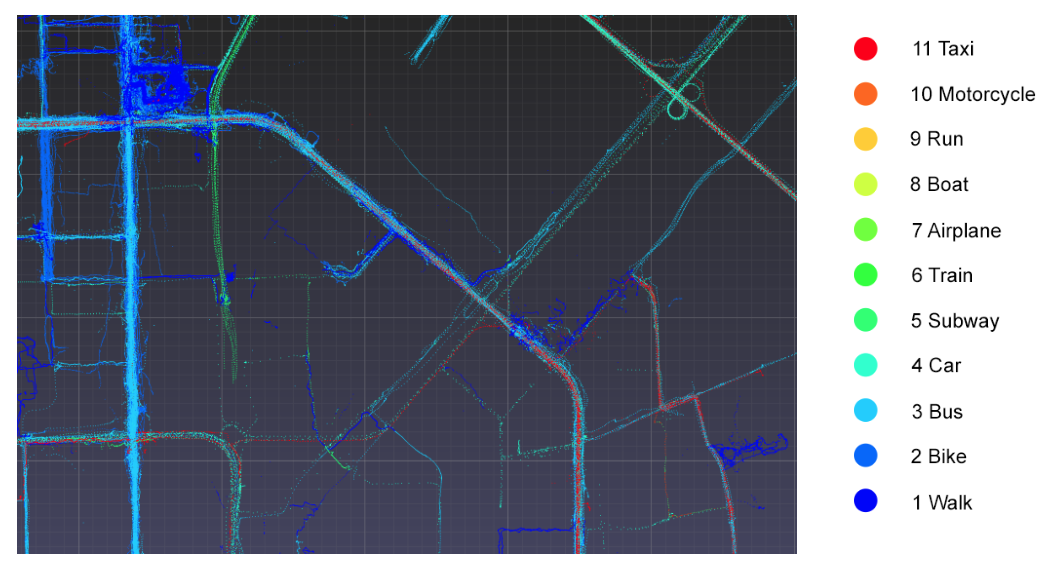
\includegraphics[width=1\textwidth]{images/tul-cls.png}
\caption{Transportation Mode Identification} 
\end{figure}
\end{columns}

\end{frame}


\begin{frame}
\frametitle{Problem of TMI}
\alert{However, existing TMI approaches have relied heavily on the availability of transportation mode labels, which is often limited in real-world applications.}

\begin{itemize}
 \item Training highly accurate deep learning models primarily requires immense amounts of data.
 \item Existing TMI research typically employs machine or deep learning models in fully supervised settings, thereby assuming the availability of sufficient GPS trajectories labeled by transportation mode at training time.
\end{itemize}

\end{frame}

\begin{frame}
\frametitle{Problem of TMI}
Data crowdsourcing seeks to alleviate this issue by allowing multiple users to collectively generate large data sets in a distributed manner. A centralized server is always set to receive the crowdsourced data and train them. These data are usually transmitted to the centralized server in unprocessed forms. \alert{However, information implied by the data may have a strong connection to the users’ privacy, which raises a privacy concern.}

\end{frame}

\begin{frame}
\frametitle{Contributions}
The main contributions of this article are summarized as follows.

\begin{itemize}
 \item They propose MTSSFL, a new FL-based semi-supervised learning scheme that incorporates an ensemble-learningbased TMI model.
 \item They introduce consistency updating, a novel approach for training local models that only possess unlabeled data guided by the centralized model trained on few labeled data.
 \item They design an exponential moving average (EMA)-based secure parameter aggregation mechanism termed meanteacher-averaging to improve the global model without additional training.
 \item They conduct extensive case studies to assess the performance of MTSSFL on IID and non-IID data. 
\end{itemize}

\end{frame}


%insert preliminaries--------------------------
\section{Preliminaries}
% 1
\begin{frame}
\frametitle{GPS-Based Transportation Mode Identification}

\begin{definition}[GPS Segment]
Let $\mathcal{F}_i$ denote the calculated features of the ith GPS point in a segment. We can then reform GPS segment $k$ of length $T$ as $\mathrm{GPS}_k=\left\{\mathcal{F}_1, \mathcal{F}_2, \ldots, \mathcal{F}_T\right.$, ${label}_{k}$\}, where ${label}_{k}$ is the corresponding transportation mode of the segment. Our aim is to train a deep learning classifier to classify $\mathrm{GPS}_k, \forall k$, by transportation mode. This is formulated as
$$
\mathrm{GPS}_k\left[\mathcal{F}_1, \mathcal{F}_2, \ldots, \mathcal{F}_T\right] \stackrel{f(\cdot)}{\longrightarrow} \mathrm{GPS}_k\left[\text { label }_k\right]
$$
where $f(\cdot)$ denotes the classification function learned by the classifier model.
\end{definition}
\end{frame}

% 2
\begin{frame}
{Semisupervised Federated Learning}
{1. Crowdsourced Federated Learning Framework}
In this work, we propose an FL framework for crowdsourced TMI. We use the term “publisher” to refer to the initiator of the crowdsourcing task, who also owns a central server. We refer to the local (distributed) entities as “workers.”
\begin{block}{Statement}
Let $q$ denote the total number of workers; we then have the set of workers $\mathcal{C}=\left\{C_1, C_2, \ldots, C_q\right\}$. Each worker $C_i$ uses their respective database $D_i$ to store their sensed GPS trajectories, resulting in the database set $\mathcal{D}=\left\{D_1, D_2, \ldots, D_q\right\}$. In FL, worker $C_i$ uses their locally stored data to train their local $\operatorname{model} M_i \in$ $\mathcal{M}=\left\{M_1, M_2, \ldots, M_q\right\}$, where the learned parameters of $M_i$ are denoted by $\phi_i$.
\footnote{This work assumes that both the publisher and the workers are reliable and low-latency communicators.}
\end{block}

\end{frame}

\begin{frame}
{Semisupervised Federated Learning}
{2. IID and Non-IID Data}
Each worker is likely to have more data corresponding to some transportation modes than others. This will inevitably lead to a skewed local class distribution, i.e., nonindependent and identically distributed (non-IID) data.

\begin{definition}[The metric R to measure the level of non-IID]
Specifically, the class distribution of database $D_i$ belonging to worker $C_i$ is defined as $P_i=\left[p_1, p_2, \ldots, p_c\right] \in \mathbb{R}^c$, where $p_j$ is the fraction of the $j$ th class in $D_i$ and $c$ denotes the total number of classes. $R$ can be defined as
$$
R=\frac{1}{2} \sum_{1 \leq i<o \leq q}\left\|P_i-P_o\right\|_1 \frac{1}{q(q-1) / 2}
$$
where $\|\cdot\|_1$ denotes the $L_1$ norm, $\left\|P_i-P_o\right\|_1$ is the variation distance, and $q(q-1) / 2$ corresponds to the total number of worker pairs. 
\end{definition}
\end{frame}

% insert methodology -----------------------------------
\section{Methodology}
% 1
\begin{frame}
{Representation of TMI Data Features}
{GPS Trajectory Preprocessing}
This segmentation method is based on the intuition that \alert{the transportation mode separating any other two has to be walk.}

%\\\

As such, this method first classifies each GPS point as walk or nonwalk according to velocity and acceleration thresholds before forming single-transportation-mode segments by aggregating adjacent points with the same predicted label. 

Using the same thresholds defined by \footnote{TY. Zheng, L. Liu, L. Wang, and X. Xie, “Learning transportation mode from raw GPS data for geographic applications on the Web,” in Proc. 17th Int. Conf. World Wide Web, 2008, pp. 247–256.}, we split all trajectories into a total of $T^*$ single-transportation-mode segments \{GPS$_1$, GPS$_2 \ldots$, GPS $\left._{T^*}\right\}$


%\begin{block}{}
%[1] Y. Zheng, L. Liu, L. Wang, and X. Xie, “Learning transportation mode from raw GPS data for geographic applications on the Web,” in Proc. 17th Int. Conf. World Wide Web, 2008, pp. 247–256.
%\end{block}
\end{frame}



\begin{frame}
{Representation of TMI Data Features}
{Motion Feature Extraction}
We first calculate the relative distance between every two consecutive GPS records using the Vincenty Formula, which can be denoted as
$$
d_i=\text { Vincenty }\left(\operatorname{lat}_i, \operatorname{lng}_i ; \operatorname{lat}_{i+1}, \operatorname{lng}_{i+1}\right)
$$

Based on $d_i$, we can then estimate speed $s_i$, acceleration $a_i$, and jerk $j_i$ for the $i$ th GPS point as follows:
$$
\begin{aligned}
&s_i=\frac{d_i}{\Delta t_i}, \quad 1 \leq i \leq T, \quad s_T=s_{T-1} \\
&a_i=\frac{s_{i+1}-s_i}{\Delta t_i}, \quad 1 \leq i \leq T, \quad a_T=0 \\
&j_i=\frac{a_{i+1}-a_i}{\Delta t_i}, \quad 1 \leq i \leq T, \quad j_T=0
\end{aligned}
$$
where $T$ is the number of GPS records in a GPS segment. In this way, a motion feature vector $x_i \equiv \mathcal{F}_i=\left(d_i, s_i, a_i, j_i\right)$ can be extracted for the ith GPS point. 
\end{frame}

% 2
\begin{frame}
{TMI Model}
{Overview}
\begin{figure}[ht]
\centering
\includegraphics[height=0.56\textwidth]{images/tmi}
\caption{Framework of TMI model.} 
\end{figure}
\end{frame}

\begin{frame}
{TMI Model}
{Feature Extraction}
{Model 1}

This submodel first employs three convolution layers with skip connections to capture the spatial features within the input motion features $\mathbf{X}$. Next, we stack eight layers of gated recurrent units (GRUs) with hidden size 16 to exploit the temporal dependencies within the input data.

\begin{columns}
\column{0.42\textwidth}
\begin{block}{Gated Recurrent Units (GRU)}
$\begin{aligned} r_t &=\sigma\left(W^{(r)} \mathbf{X}_t+U^{(r)} h_{t-1}\right) \\ z_t &=\sigma\left(W^{(z)} \mathbf{X}_t+U^{(z)} h_{t-1}\right) \\ h_t^{\prime} &=\tanh \left(W \mathbf{X}_t+r_t \odot U h_{t-1}\right) \\ h_t &=z^t \odot h_{t-1}+\left(1-z_t\right) \odot \tilde{h}_t \end{aligned}$
\end{block}
\column{0.38\textwidth}
\begin{figure}[ht]
\centering
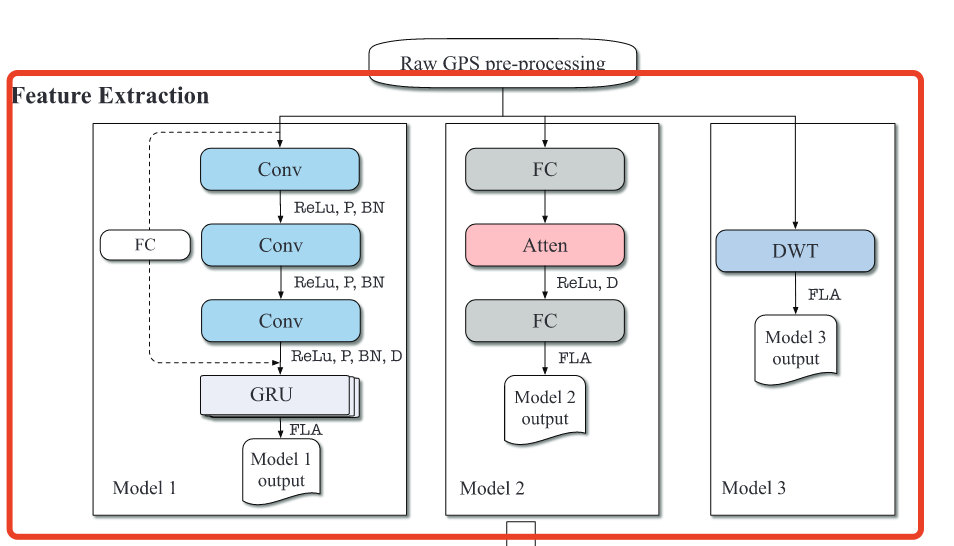
\includegraphics[height=0.67\textwidth]{images/feature}
\caption{Framework of TMI model.} 
\end{figure}
\end{columns}
\end{frame}

\begin{frame}
{TMI Model}
{Feature Extraction}
{Model 2}

This submodel incorporates an attention module between two linear layers.

The orchestra of multihead enables the model to collectively involve knowledge learned from multiple representation subspaces. The processes can be formulated as
$$
\mathbf{X}^A=\operatorname{concat}\left(h d_1, h d_2, \ldots, h d_{n^*}\right) W^O
$$
where
$$
h d_i=\operatorname{softmax}\left(\frac{Q W_i^Q\left(K W_i^K\right)^T}{\sqrt{d_k}}\right) V W_i^V
$$
where $Q, K$, and $V$ are the query, key, and value, and the mechanism requires that they are all $\mathbf{X} ; d_k=\left(h i d d_a / n^*\right)$ denotes the dimension of keys where $\operatorname{hidd}_a$ denotes the hidden size of the attention module, which is set to 128 ; $h d_i$ denotes each attentional head and $n^*$ is the number of heads; concat $(\cdot)$ represents the concatenation operation; $W^O, W^Q, W^K$, and $W^V$ are the corresponding weight matrices.
\end{frame}

\begin{frame}
{TMI Model}
{Feature Extraction}
{Model 3}

To better analyze the data characteristics, a wavelet representation-based feature extracting approach named discrete wavelet transform (DWT) is adopted in Model 3 to further exploit the hidden time-domain feature from the feature vectors.

Specifically, DWT employs discrete wavelets $\psi_{a, b}(t)$ to convolve the input, which can be defined as
$$
\psi_{a, b}(t)=\frac{1}{2^a} \psi\left(\frac{t}{2^a}-b\right), a, b \in \mathbb{Z}
$$
where $\psi(t)$ is predefined mother wavelet, $a$ denotes the oscillatory level, and $b$ denotes the shifted position of DWT. 
\end{frame}

\begin{frame}
{TMI Model}
{Ensembling}
Multiview ensemble learning (MEL) is a type of semisupervised learning aiming to train different learning models with \alert{different views of the original data.}
Following the concept of MEL, we create four ensembles by concatenating the outputs of the three submodels as:

$$
\begin{aligned}
&\mathbf{X}^{E 1}=\operatorname{concat}\left(\mathbf{X}^{M 1}, \mathbf{X}^{M 2}, \mathbf{X}^{M 3}\right) \\
&\mathbf{X}^{E 2}=\operatorname{concat}\left(\mathbf{X}^{M 1}, \mathbf{X}^{M 2}\right) \\
&\mathbf{X}^{E 3}=\operatorname{concat}\left(\mathbf{X}^{M 1}, \mathbf{X}^{M 3}\right) \\
&\mathbf{X}^{E 4}=\operatorname{concat}\left(\mathbf{X}^{M 2}, \mathbf{X}^{M 3}\right)
\end{aligned}
$$ 
where $\mathbf{X}^{M 1}, \mathbf{X}^{M 2}$, and $\mathbf{X}^{M 3}$ are the outputs of the three submodels; $\mathbf{X}^{E 1}, \mathbf{X}^{E 2}, \mathbf{X}^{E 3}$, and $\mathbf{X}^{E 4}$ denote the four ensemble tensors for corresponding ensembles.
\end{frame}

\begin{frame}
{TMI Model}
{Voting}
Finally, we use a voting strategy to decide the final transportation mode classification from the predictions of the four ensembles. 

Specifically, we regard the inferred transportation mode of each ensemble as a candidate. \alert{A hard voting procedure} is adopted, in which we select the final class as the one with the largest sum of votes among the classes predicted by the four candidates. In the case of a tie, we consider the transportation mode classification provided by Ensemble 1 as the final classification, since Ensemble 1 is trained on more inputs and is thus expected to be more reliable than the others.
\end{frame}

% 3
\begin{frame}
{Mean Teacher Semisupervised Federated Learning}
{Architecture, Participants, and Communication Protocol}

\begin{figure}[ht]
\centering
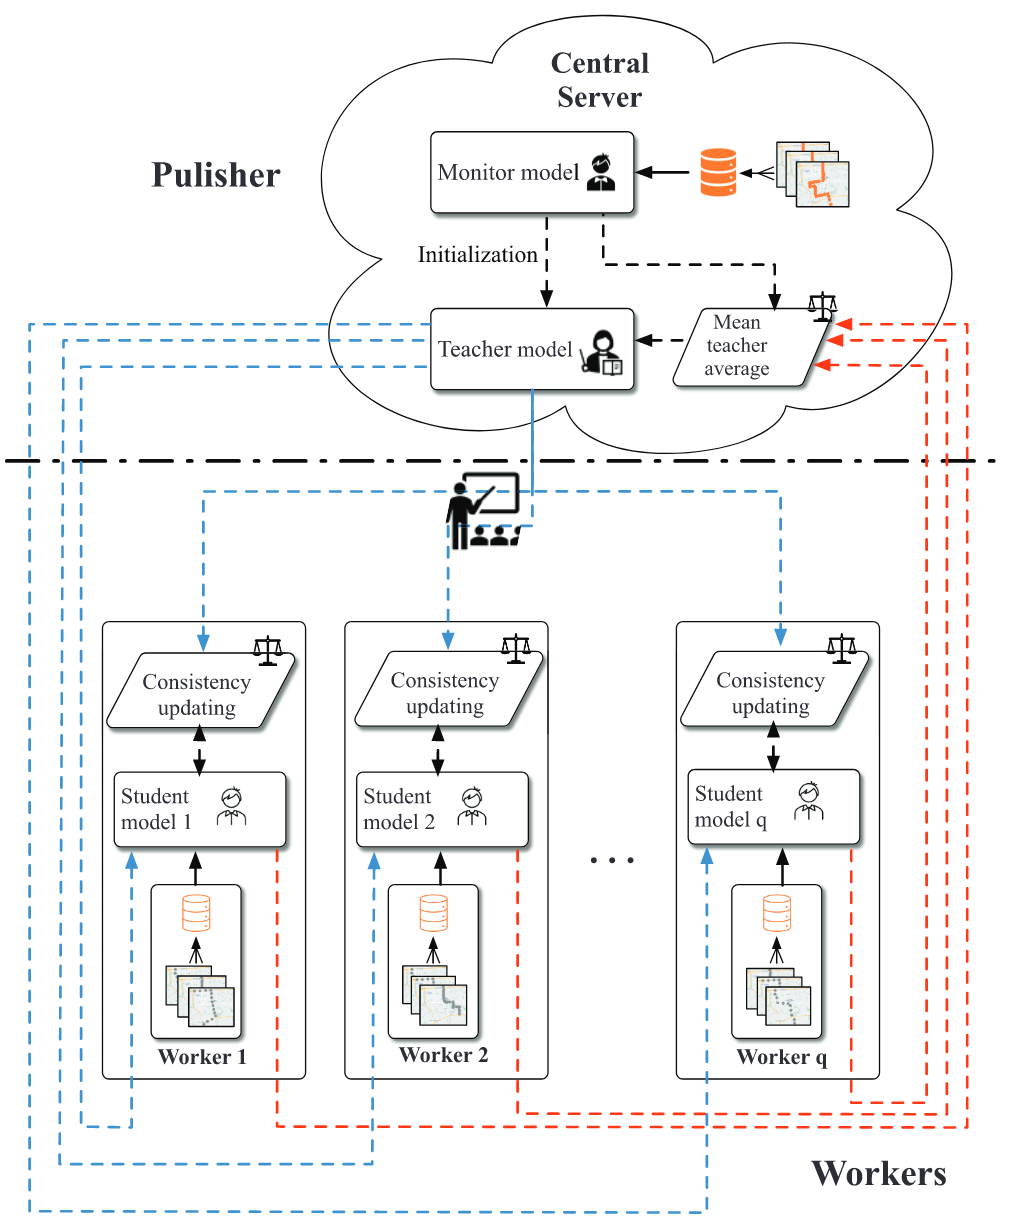
\includegraphics[height=0.54\textwidth]{images/fl}
\caption{Framework overview of the proposed MTSSFL.} 
\end{figure}
\end{frame}

\begin{frame}
{Mean Teacher Semisupervised Federated Learning}
{Consistency Updating}
{Pseudolabeling Approach}

The pseudolabeling approach considers the training balance between labeled data and unlabeled data, which defines a loss function as
\begin{equation}
J=\frac{1}{B} \sum_{m=1}^B \sum_{i=1}^c J\left(y_i^m, \hat{y}_i^m\right)+\alpha(t) \frac{1}{B^{\prime}} \sum_{m=1}^{B^{\prime}} \sum_{i=1}^c J\left(y_i^{\prime m}, \hat{y}_i^{\prime m}\right)
\end{equation}
where $B$ and $B^{\prime}$ denote the size of minibatch in labeled and unlabeled data, respectively; $\hat{y}_i^m$ and $\hat{y}_i^{\prime m}$ are the output of $m$ samples in labeled and unlabeled data, respectively; $y_i^m$ and $y_i^{\prime m}$ are the labels of $m$ samples in labeled and unlabeled data, respectively; $\alpha(t)$ is a balancing weight.

\end{frame}


\begin{frame}
{Mean Teacher Semisupervised Federated Learning}
{Consistency Updating}

A consistency cost $J_{\text {con }}$ is introduced to measure the distance between the prediction of student model and teacher model on unlabeled data using L2 loss, which can be formulated as

\begin{equation}
J_{\mathrm{con}}=\frac{1}{c} \sum_{i=1}^c\left(\dot{f}\left(x_i^{\prime m}\right)-f\left(x_i^{\prime m}\right)\right)^2
\end{equation}

where $\dot{f}$ and $f$ denote the teacher and student TMI model, respectively; $x_i^{\prime m}$ is the unlabeled data. Furthermore, we can define a final loss function $J_s$ for the student model's update by combining (1) and the second half of the (2), which can be formulated as

\begin{equation}
J_s=\frac{1}{B^{\prime}} \sum_{m=1}^{B^{\prime}} J_{\mathrm{con}}+\frac{1}{B^{\prime}} \sum_{m=1}^{B^{\prime}} \sum_{i=1}^c J\left(y_i^{\prime m}, f\left(x_i^{\prime m}\right)\right)
\end{equation}

\end{frame}

\begin{frame}
{Mean Teacher Semisupervised Federated Learning}
{Mean-Teacher-Averaging}
In this work, we proposed a mean-teacher-averaging as a secure parameter aggregation mechanism for the TMI models based on the approach proposed in \footnote{A. Tarvainen and H. Valpola, “Mean teachers are better role models: Weight-averaged consistency targets improve semi-supervised deep learning results,” in Advances in Neural Information Processing Systems. Red Hook, NY, USA: Curran, 2017, pp. 1195–1204.}.
Tarvainen and Valpola  proposed an \alert{EMA-based} approach to update the model parameter of the teacher model at communication round $t$, which can be defined as
\begin{equation}
	\dot{\phi}_t=\delta \dot{\phi}_{t-1}+(1-\delta) \phi_t
\end{equation}

where $\dot{\phi}$ and $\phi$ are the parameters of teacher model and student model, respectively; and $\delta$ is a smoothing coefficient.

%\begin{block}{}
%[2] A. Tarvainen and H. Valpola, “Mean teachers are better role models: Weight-averaged consistency targets improve semi-supervised deep learning results,” in Advances in Neural Information Processing Systems. Red Hook, NY, USA: Curran, 2017, pp. 1195–1204.
%\end{block}
\end{frame}

\begin{frame}
{Mean Teacher Semisupervised Federated Learning}
{Mean-Teacher-Averaging}

We extend this method into a model parameter aggregation method applicable to FL. Specifically, we first use the naive FedAvg [56] to aggregate model updates of student and monitor models, which can be formulated as
\begin{equation}
	\phi_{\Sigma, t}=\frac{1}{1+q}\left(\sum_{i=1}^q \phi_{i, t}+\ddot{\phi}_t\right)
\end{equation}
where $q$ denotes the number of student models (i.e., workers); $\ddot{\phi}$ is the model parameter of monitor model; and $\phi_{\Sigma}$ represents the aggregated parameters from student and monitor models by FedAvg. Subsequently, we incorporate $\phi_{\Sigma}$ by (4) into (5), and finally, obtain the aggregation mechanism for MTSSFL as
\begin{equation}
\dot{\phi}_t=\delta \dot{\phi}_{t-1}+(1-\delta) \phi_{\Sigma, t} .
\end{equation}
\end{frame}



% insert Experiments -----------------------------------
\section{Experiments}

% 1
\begin{frame}
{Experimental Setup}
{Data Set Description}
{Geolife}

An open data set of real-world GPS trajectories by Microsoft Research Asia. It contains a total of 17 621 trajectories collected by 182 users over 2090 days, with a total traveled distance of 1 292 951 km. Among these users, only 69 have labeled parts of their trajectories by transportation mode.

\end{frame}

\begin{frame}
{Experimental Setup}
{Experimental Settings}
Our simulations were conducted on a server equipped with eight NVIDIA GeForce RTX 2080 GPUs and an Intel Xeon E5-2620 v4 CPU. All neural networks were developed using PyTorch v1.6.
\end{frame}

% 2
\begin{frame}
{Identification Accuracy}
{Results}
\begin{table}
\caption{Comparision of TMI Methods}
\begin{tabular}{lccc}
\hline Method & Accuracy & Semi-supervised & Secure crowdsourcing \\
\hline MLP & $33.1 \%$ & $-$ & $-$ \\
SVM & $47.0 \%$ & $-$ & $-$ \\
KNN & $54.9 \%$ & $-$ & $-$ \\
CNN & $83.6 \%$ & $-$ & $-$ \\
LSTM & $81.7 \%$ & $-$ & $-$ \\
SPL & $72.5 \%$ & $\checkmark$ & $-$ \\
SGAN & $83.1 \%$ & $\checkmark$ & $-$ \\
SECA & $73.2 \%$ & $\checkmark$ & $-$ \\
STS & $59.1 \%$ & $\checkmark$ & $-$ \\
ELSTM & $90.3 \%$ & $\checkmark$ & $-$ \\
\bf{MTSSFL} & $89.2 \%$ & $\checkmark$ & $\checkmark$ \\
\hline
\end{tabular}
\end{table}

\end{frame}

\begin{frame}
{Identification Accuracy}
{Accuracy for Different Percentages of Unlabeled Data}

\begin{table}
\caption{Sensitivity of TMI Accuracy to Percentage of Unlabeled Data}
\resizebox{\linewidth}{!}{
\begin{tabular}{lcccccc}
\hline \multirow{2}{*}{ Method } & \multicolumn{6}{c}{ Accuracy (\%) } \\
\cline { 2 - 7 } & $\gamma=0.99$ & $\gamma=0.95$ & $\gamma=0.90$ & $\gamma=0.80$ & $\gamma=0.50$ & $\gamma=0$ (Supervised) \\
\hline SPL & $50.9$ & $56.0$ & $61.8$ & $68.6$ & $72.5$ & $75.4$ \\
SGAN & $68.4$ & $77.7$ & $80.5$ & $82.1$ & $83.1$ & $83.8$ \\
SECA & $52.0$ & $56.1$ & $62.9$ & $69.3$ & $73.2$ & $76.8$ \\
STS & $50.7$ & 53 & $50.6$ & $54.4$ & $57.7$ & $59.1$ \\
ELSTM & $84.8$ & $86.5$ & $89.0$ & $90.0$ & $90.8$ & $91.5$ \\
\bf{MTSSFL} & $82.4$ & $83.1$ & $85.7$ & $87.3$ & $89.2$ & $91.4$ \\
\bf{MTSSFL-non-IID} & $82.3$ & $82.5$ & $85.7$ & $86.9$ & $89.0$ & $91.3$ \\
\hline
\end{tabular}
}
\end{table}
\end{frame}


\begin{frame}
{Identification Accuracy}
\begin{table}
\caption{Accuracy and Training Time of MTSSFL for Different Numbers of Local Epochs}
\begin{tabular}{ccc}
\hline$E_l$ & Accuracy (\%) & Training time (s) \\
\hline 1 & $89.1$ & $750 \pm 30$ \\
2 & $88.9$ & $1480 \pm 30$ \\
3 & $88.8$ & $1920 \pm 45$ \\
4 & $88.3$ & $2620 \pm 70$ \\
5 & $89.2$ & $3110 \pm 80$ \\
\hline
\end{tabular}
\end{table}

\end{frame}



%\section{Conclusions}
%\begin{frame}
%\frametitle{Two-column slide}
%\end{frame}

% Insert a thank your frame ------------------------------------------------
\begin{frame}
\Huge{\centerline{Thank you!}}
\end{frame}

\end{document}